\subsection{$B_s$-Mixing}
\begin{figure}[t]
 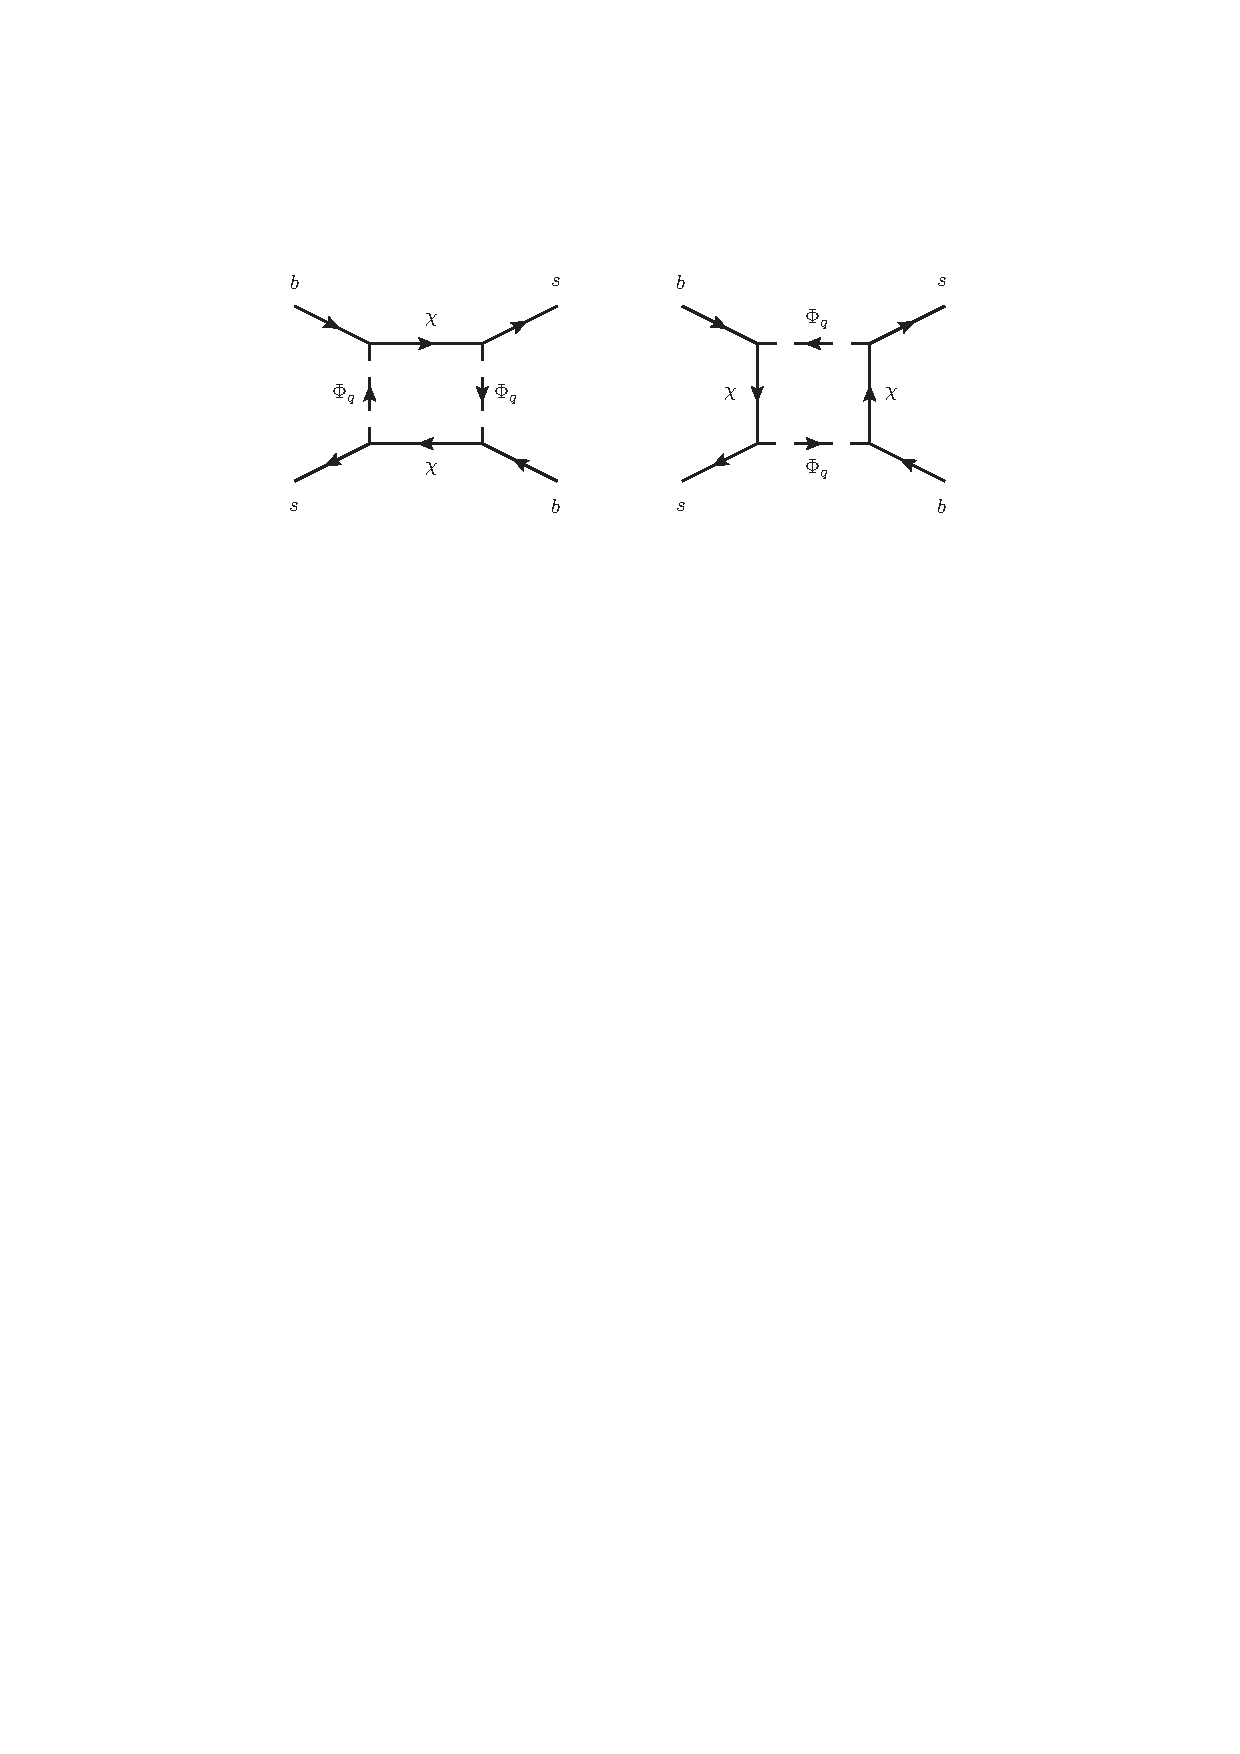
\includegraphics[width=1\textwidth]{../pics/bsmix.pdf}
 \caption{$B_s$-mixing. The crossed boxes also occur, see fig. \ref{pic_Bsmumu}}
 \label{pic_Bsmix}
\end{figure}
As the semileptonic meson decays, hadronic ones are accordingly enabled. The diagrams for $B_s$-mixing are depicted in figure \ref{pic_Bsmix}. 
The parameter set consists of
\begin{align}
 \left\{m_\chi,M_q\right\}.
\end{align}
Other
meson mixings like $K\bar K$ or $ D \bar D$ are suppressed due to their smaller Yukawa couplings. From a calculational point of view, this process is 
quite similar to the former $b\rightarrow s\bar\mu\mu$ and is induced only through one-loop box diagrams in the SM to the lowest order. The effective Hamiltonian
involves only one operator $(\bar s \gamma^\mu P_L b)(\bar s \gamma_\mu P_L b)$ for our chiral theory whose Wilson coefficient reads
\begin{align}
 C_{B\bar B}^1 &=  \frac{|g_2^{q*}g_3^q|^2}{m_\chi^2} \frac{1}{128\pi^2} \left(K'(x_q) + 2 G'(x_q)\right)\label{eq_WilsonMix1}\\
 C_{B\bar B}^3 &=  \frac{|g_2^{q*}g_3^q|^2}{m_\chi^2} \frac{5}{384\pi^2} \left(K'(x_q) + 2\cdot\frac15 G'(x_q)\right)
 \label{eq_WilsonMix3}
\end{align}
with the first derivatives $K'(x)$ and $G'(x)$ \eqref{eq_mixloops} being the limits of $K(x,y)$ and $G(x,y)$, respectively, for $y\rightarrow x$. 

